\documentclass[
  man,
  floatsintext,
  longtable,
  nolmodern,
  notxfonts,
  notimes,
  colorlinks=true,linkcolor=blue,citecolor=blue,urlcolor=blue]{apa7}

\usepackage{amsmath}
\usepackage{amssymb}



\usepackage[bidi=default]{babel}
\babelprovide[main,import]{english}


% get rid of language-specific shorthands (see #6817):
\let\LanguageShortHands\languageshorthands
\def\languageshorthands#1{}

\RequirePackage{longtable}
\RequirePackage{threeparttablex}

\makeatletter
\renewcommand{\paragraph}{\@startsection{paragraph}{4}{\parindent}%
	{0\baselineskip \@plus 0.2ex \@minus 0.2ex}%
	{-.5em}%
	{\normalfont\normalsize\bfseries\typesectitle}}

\renewcommand{\subparagraph}[1]{\@startsection{subparagraph}{5}{0.5em}%
	{0\baselineskip \@plus 0.2ex \@minus 0.2ex}%
	{-\z@\relax}%
	{\normalfont\normalsize\bfseries\itshape\hspace{\parindent}{#1}\textit{\addperi}}{\relax}}
\makeatother




\usepackage{longtable, booktabs, multirow, multicol, colortbl, hhline, caption, array, float, xpatch}
\setcounter{topnumber}{2}
\setcounter{bottomnumber}{2}
\setcounter{totalnumber}{4}
\renewcommand{\topfraction}{0.85}
\renewcommand{\bottomfraction}{0.85}
\renewcommand{\textfraction}{0.15}
\renewcommand{\floatpagefraction}{0.7}

\usepackage{tcolorbox}
\tcbuselibrary{listings,theorems, breakable, skins}
\usepackage{fontawesome5}

\definecolor{quarto-callout-color}{HTML}{909090}
\definecolor{quarto-callout-note-color}{HTML}{0758E5}
\definecolor{quarto-callout-important-color}{HTML}{CC1914}
\definecolor{quarto-callout-warning-color}{HTML}{EB9113}
\definecolor{quarto-callout-tip-color}{HTML}{00A047}
\definecolor{quarto-callout-caution-color}{HTML}{FC5300}
\definecolor{quarto-callout-color-frame}{HTML}{ACACAC}
\definecolor{quarto-callout-note-color-frame}{HTML}{4582EC}
\definecolor{quarto-callout-important-color-frame}{HTML}{D9534F}
\definecolor{quarto-callout-warning-color-frame}{HTML}{F0AD4E}
\definecolor{quarto-callout-tip-color-frame}{HTML}{02B875}
\definecolor{quarto-callout-caution-color-frame}{HTML}{FD7E14}

%\newlength\Oldarrayrulewidth
%\newlength\Oldtabcolsep


\usepackage{hyperref}




\providecommand{\tightlist}{%
  \setlength{\itemsep}{0pt}\setlength{\parskip}{0pt}}
\usepackage{longtable,booktabs,array}
\usepackage{calc} % for calculating minipage widths
% Correct order of tables after \paragraph or \subparagraph
\usepackage{etoolbox}
\makeatletter
\patchcmd\longtable{\par}{\if@noskipsec\mbox{}\fi\par}{}{}
\makeatother
% Allow footnotes in longtable head/foot
\IfFileExists{footnotehyper.sty}{\usepackage{footnotehyper}}{\usepackage{footnote}}
\makesavenoteenv{longtable}

\usepackage{graphicx}
\makeatletter
\def\maxwidth{\ifdim\Gin@nat@width>\linewidth\linewidth\else\Gin@nat@width\fi}
\def\maxheight{\ifdim\Gin@nat@height>\textheight\textheight\else\Gin@nat@height\fi}
\makeatother
% Scale images if necessary, so that they will not overflow the page
% margins by default, and it is still possible to overwrite the defaults
% using explicit options in \includegraphics[width, height, ...]{}
\setkeys{Gin}{width=\maxwidth,height=\maxheight,keepaspectratio}
% Set default figure placement to htbp
\makeatletter
\def\fps@figure{htbp}
\makeatother


% definitions for citeproc citations
\NewDocumentCommand\citeproctext{}{}
\NewDocumentCommand\citeproc{mm}{%
  \begingroup\def\citeproctext{#2}\cite{#1}\endgroup}
\makeatletter
 % allow citations to break across lines
 \let\@cite@ofmt\@firstofone
 % avoid brackets around text for \cite:
 \def\@biblabel#1{}
 \def\@cite#1#2{{#1\if@tempswa , #2\fi}}
\makeatother
\newlength{\cslhangindent}
\setlength{\cslhangindent}{1.5em}
\newlength{\csllabelwidth}
\setlength{\csllabelwidth}{3em}
\newenvironment{CSLReferences}[2] % #1 hanging-indent, #2 entry-spacing
 {\begin{list}{}{%
  \setlength{\itemindent}{0pt}
  \setlength{\leftmargin}{0pt}
  \setlength{\parsep}{0pt}
  % turn on hanging indent if param 1 is 1
  \ifodd #1
   \setlength{\leftmargin}{\cslhangindent}
   \setlength{\itemindent}{-1\cslhangindent}
  \fi
  % set entry spacing
  \setlength{\itemsep}{#2\baselineskip}}}
 {\end{list}}
\usepackage{calc}
\newcommand{\CSLBlock}[1]{\hfill\break\parbox[t]{\linewidth}{\strut\ignorespaces#1\strut}}
\newcommand{\CSLLeftMargin}[1]{\parbox[t]{\csllabelwidth}{\strut#1\strut}}
\newcommand{\CSLRightInline}[1]{\parbox[t]{\linewidth - \csllabelwidth}{\strut#1\strut}}
\newcommand{\CSLIndent}[1]{\hspace{\cslhangindent}#1}





\usepackage{newtx}

\defaultfontfeatures{Scale=MatchLowercase}
\defaultfontfeatures[\rmfamily]{Ligatures=TeX,Scale=1}





\title{Label Effects on Perceptions and Behaviors Toward Unhoused
Individuals}


\shorttitle{Label Effects and Homlessness}


\usepackage{etoolbox}






\author{Huidi Yuan}



\affiliation{
{University of Chicago}}




\leftheader{Yuan}



\abstract{This study investigates how inclusive labels, compared to
stigmatizing terms, shape public perceptions and prosocial behaviors
toward unhoused individuals. Drawing on theories of labeling and stigma,
we hypothesized that person-centered labels (e.g., ``people experiencing
housing insecurity'') would reduce stigma and stereotypes (H1) and
increase donations (H2). A preregistered online experiment with 400 U.S.
adults tested these hypotheses using a between-subjects design.
Participants viewed materials referencing either ``the homeless''
(stigmatizing label) or ``people experiencing housing insecurity''
(inclusive label). Results supported H1: PC labels significantly reduced
stigma and negative stereotypes. However, H2 was unsupported, as
donations did not differ between conditions. Stigma negatively
correlated with donation amounts, but stereotypes showed no
relationship. Exploratory analyses found no moderation by political
orientation or age. These findings highlight the potential of PC labels
to mitigate stigma, though additional strategies are needed to bridge
the gap between attitudinal and behavioral change. Implications for
advocacy, policy communication, and future research are discussed.}

\keywords{Inclusive Language, stigma, homelessness, prosocial
behavior, labeling effects}


\makeatletter
\let\endoldlt\endlongtable
\def\endlongtable{
\hline
\endoldlt
}
\makeatother

\urlstyle{same}



\usepackage{booktabs}
\usepackage{longtable}
\usepackage{array}
\usepackage{multirow}
\usepackage{wrapfig}
\usepackage{float}
\usepackage{colortbl}
\usepackage{pdflscape}
\usepackage{tabu}
\usepackage{threeparttable}
\usepackage{threeparttablex}
\usepackage[normalem]{ulem}
\usepackage{makecell}
\usepackage{xcolor}
\makeatletter
\@ifpackageloaded{caption}{}{\usepackage{caption}}
\AtBeginDocument{%
\ifdefined\contentsname
  \renewcommand*\contentsname{Table of contents}
\else
  \newcommand\contentsname{Table of contents}
\fi
\ifdefined\listfigurename
  \renewcommand*\listfigurename{List of Figures}
\else
  \newcommand\listfigurename{List of Figures}
\fi
\ifdefined\listtablename
  \renewcommand*\listtablename{List of Tables}
\else
  \newcommand\listtablename{List of Tables}
\fi
\ifdefined\figurename
  \renewcommand*\figurename{Figure}
\else
  \newcommand\figurename{Figure}
\fi
\ifdefined\tablename
  \renewcommand*\tablename{Table}
\else
  \newcommand\tablename{Table}
\fi
}
\@ifpackageloaded{float}{}{\usepackage{float}}
\floatstyle{ruled}
\@ifundefined{c@chapter}{\newfloat{codelisting}{h}{lop}}{\newfloat{codelisting}{h}{lop}[chapter]}
\floatname{codelisting}{Listing}
\newcommand*\listoflistings{\listof{codelisting}{List of Listings}}
\makeatother
\makeatletter
\makeatother
\makeatletter
\@ifpackageloaded{caption}{}{\usepackage{caption}}
\@ifpackageloaded{subcaption}{}{\usepackage{subcaption}}
\makeatother

% From https://tex.stackexchange.com/a/645996/211326
%%% apa7 doesn't want to add appendix section titles in the toc
%%% let's make it do it
\makeatletter
\xpatchcmd{\appendix}
  {\par}
  {\addcontentsline{toc}{section}{\@currentlabelname}\par}
  {}{}
\makeatother

%% Disable longtable counter
%% https://tex.stackexchange.com/a/248395/211326

\usepackage{etoolbox}

\makeatletter
\patchcmd{\LT@caption}
  {\bgroup}
  {\bgroup\global\LTpatch@captiontrue}
  {}{}
\patchcmd{\longtable}
  {\par}
  {\par\global\LTpatch@captionfalse}
  {}{}
\apptocmd{\endlongtable}
  {\ifLTpatch@caption\else\addtocounter{table}{-1}\fi}
  {}{}
\newif\ifLTpatch@caption
\makeatother

\begin{document}

\maketitle


\setcounter{secnumdepth}{-\maxdimen} % remove section numbering

\setlength\LTleft{0pt}


\section{Introduction}\label{introduction}

The way individuals are labeled---such as ``the homeless'' versus
``people who experience housing insecurity''---can influence stigma,
stereotypes, and charitable behavior. This study examines how different
labels affect:

\begin{itemize}
\tightlist
\item
  Perceptions of homelessness-related stigma,
\item
  Stereotypical judgments,
\item
  Donation behaviors.
\end{itemize}

We hypothesize that:

\begin{enumerate}
\def\labelenumi{\arabic{enumi}.}
\tightlist
\item
  Person-centered labels reduce stigma and stereotypes (H1);
\item
  Person-centered labels increase donations to unhoused group (H2);
\item
  Stigma and stereotypes predict donation amounts to unhoused group
  (H3).
\end{enumerate}

\subsection{Methods}\label{methods}

\subsubsection{Participants}\label{participants}

A total of 399 participants were recruited. 9 participants were excluded
due to failing attention checks. Thus the final sample size was 390.

\subsubsection{Measures}\label{measures}

\begin{itemize}
\tightlist
\item
  \textbf{Stigma Perception} (6-item 5-points Likert scale)
\item
  \textbf{Stereotypical Judgment} (8-item 5-points Likert scale)
  (\citeproc{ref-fiskeetal_2002_model}{Fiske et al., 2002})
\item
  \textbf{Donation Allocation} (Amount donated to homeless organizations
  out of three different organizations) See Table~\ref{tbl-measures} for
  detailed measures and items.
\end{itemize}

\begin{table}

{\caption{{Main Measures}{\label{tbl-measures}}}
\vspace{-20pt}}

\begin{longtable}[]{@{}
  >{\raggedright\arraybackslash}p{(\columnwidth - 4\tabcolsep) * \real{0.2500}}
  >{\raggedright\arraybackslash}p{(\columnwidth - 4\tabcolsep) * \real{0.2083}}
  >{\raggedright\arraybackslash}p{(\columnwidth - 4\tabcolsep) * \real{0.5417}}@{}}
\toprule\noalign{}
\begin{minipage}[b]{\linewidth}\raggedright
\end{minipage} & \begin{minipage}[b]{\linewidth}\raggedright
\textbf{Measures}
\end{minipage} & \begin{minipage}[b]{\linewidth}\raggedright
\textbf{Items}
\end{minipage} \\
\midrule\noalign{}
\endhead
\bottomrule\noalign{}
\endlastfoot
& \textbf{Stigma} \emph{N = 6} & {[}Label{]} are responsible for their
condition \\
& \emph{Likert (1-5)} & {[}Label{]} are dangerous \\
\textbf{Survey Measures} & & It is better to be away from
{[}Label{]}. \\
& \textbf{Stereotypes} \emph{N = 8} & How competent are {[}Label{]}? \\
& \emph{Likert (1-5)} & How well educated are {[}Label{]}? \\
& & How warmhearted are {[}Label{]}? \\
------------------ & --------------- &
--------------------------------------- \\
& \textbf{Donation} \emph{\$100} & Covenant House - For {[}Label{]} \\
\textbf{Behavioral Measures} & & Save the Children \\
& & American Society for the Prevention of Cruelty to Animals (ASPCA) \\
\end{longtable}

{\vspace{-20pt}
\noindent \emph{Note.} Stigma measures include: Responsibility, danger, social distance; Stereotypes measures include: Competence, warmth, status, competition.}

\end{table}

\section{Result}\label{result}

\subsection{Person-Centered Labels Reduce Stigma and Stereotypes
(H1)}\label{person-centered-labels-reduce-stigma-and-stereotypes-h1}

\subsubsection{Stigma}\label{stigma}

Stigma perception significantly differed by label \(F\)(1, 388) = 8.24,
\(p\) = = .004.

\begin{figure}

\caption{\label{fig-stigma-by-label}Stigma: Conventional vs.~Inclusive
Labels}

\centering{

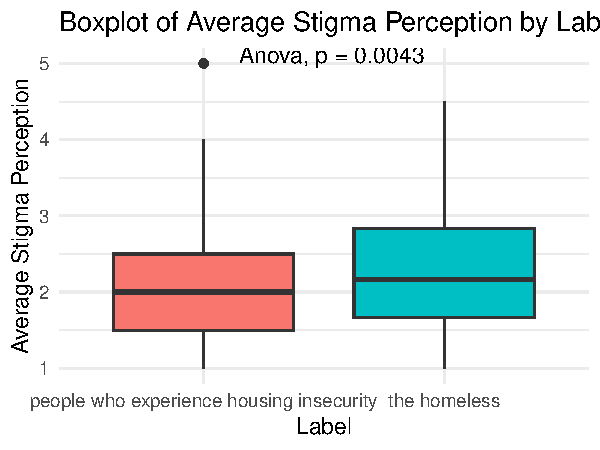
\includegraphics{00_PC_Label_Homeless_Results_files/figure-pdf/fig-stigma-by-label-1.pdf}

}

\end{figure}%

\subsubsection{Stereotypes}\label{stereotypes}

Stereotype perception significantly differed by label \(F\)(1, 388) =
7.43, \(p\) = = .007.

\begin{figure}

\caption{\label{fig-stereotype-by-label}Stereotype: Conventional
vs.~Inclusive Labels}

\centering{

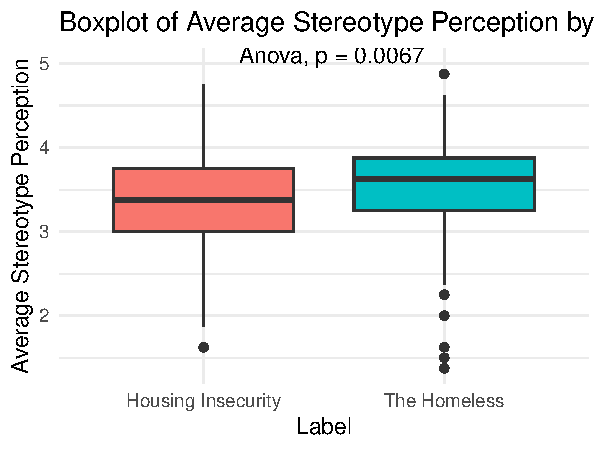
\includegraphics{00_PC_Label_Homeless_Results_files/figure-pdf/fig-stereotype-by-label-1.pdf}

}

\end{figure}%

\subsubsection{Stigma and Stereotypes
Correlation}\label{stigma-and-stereotypes-correlation}

Stigma and stereotypes were significantly correlated.

\begin{figure}

\caption{\label{fig-correlation-stigma-stereotype}Stigma
vs.~Stereotypes}

\centering{

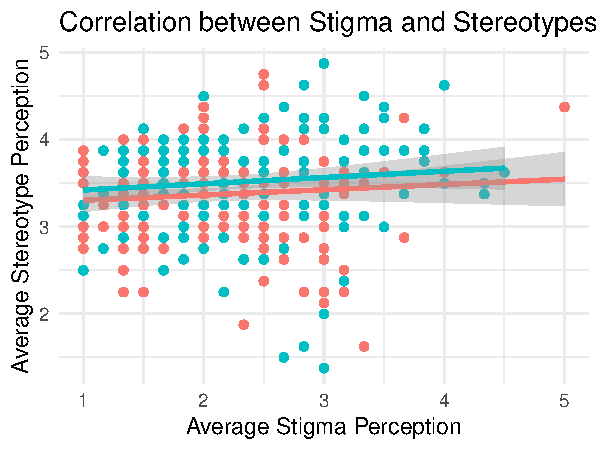
\includegraphics{00_PC_Label_Homeless_Results_files/figure-pdf/fig-correlation-stigma-stereotype-1.pdf}

}

\end{figure}%

\subsection{H2: Person-Centered Labels
vs.~Donations}\label{h2-person-centered-labels-vs.-donations}

\subsubsection{Donation Distribution}\label{donation-distribution}

Among the three organizations, avergae donation to the unhoused
organization is the highest (report mean donation to unhoused) compared
to children (report mean donation to children) and animal (report mean
donation to animal) organizations. See figure\ldots{}

\subsubsection{Donation to Unhoused Org. by
Label}\label{donation-to-unhoused-org.-by-label}

Donation, however, did not significantly differ by label \(F\)(1, 388) =
0.71, \(p\) = = .402. {[}report mean donation for unhoused org. by
label{]}

\begin{figure}

\caption{\label{fig-donate-all-by-label}Donation Distribution by Label}

\centering{

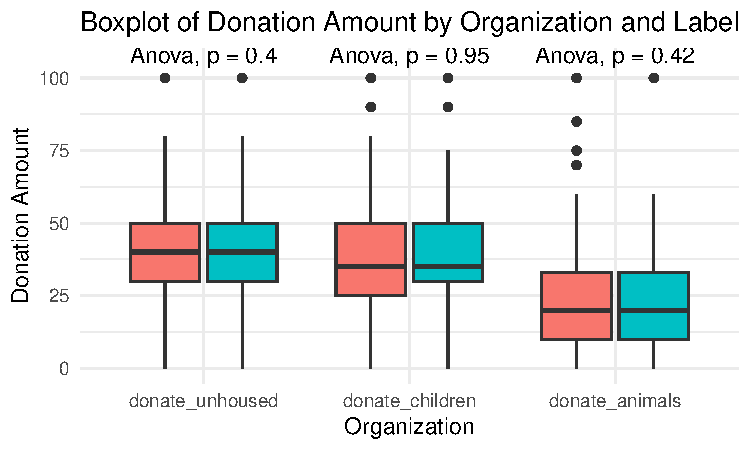
\includegraphics{00_PC_Label_Homeless_Results_files/figure-pdf/fig-donate-all-by-label-1.pdf}

}

\end{figure}%

\subsection{Stigma and stereotypes predict donation
(H3)}\label{stigma-and-stereotypes-predict-donation-h3}

\subsubsection{Stigma and Donation}\label{stigma-and-donation}

Stigma perception is negatively correlated with donation amount.
However, the relationship between stigma and donation did not differ by
label.

\begin{figure}

\caption{\label{fig-correlation-stigma-donation}Stigma vs.~Donation}

\centering{

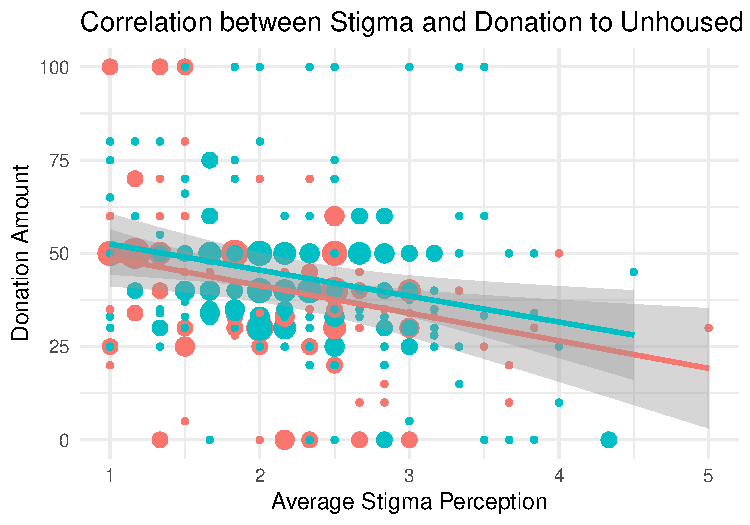
\includegraphics{00_PC_Label_Homeless_Results_files/figure-pdf/fig-correlation-stigma-donation-1.pdf}

}

\end{figure}%

\subsubsection{Stereotypes and Donation}\label{stereotypes-and-donation}

Stereotype perception is not significantly correlated with donation
amount.

\subsubsection{Exploratory Analysis}\label{exploratory-analysis}

\begin{figure}

\caption{\label{fig-donate-political-by-label}Donation by Political
Orientation and Label}

\centering{

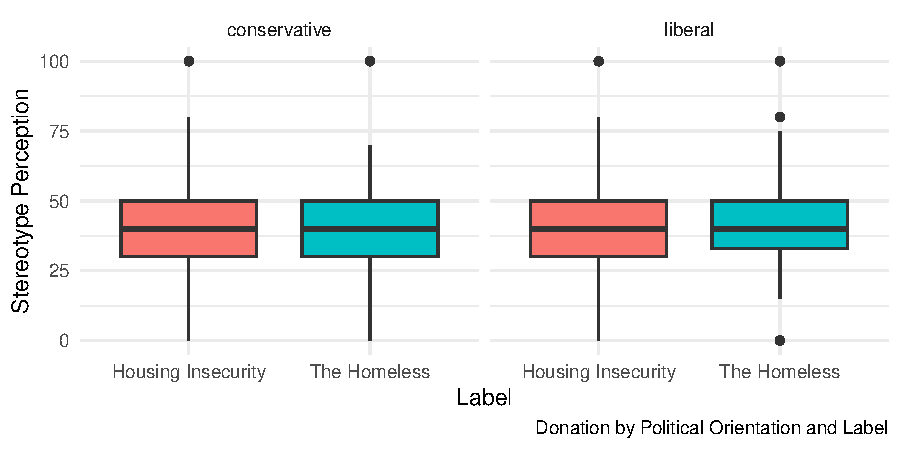
\includegraphics{00_PC_Label_Homeless_Results_files/figure-pdf/fig-donate-political-by-label-1.pdf}

}

\end{figure}%

\begin{figure}

\caption{\label{fig-donate-age-by-label}Donation by Age Group and Label}

\centering{

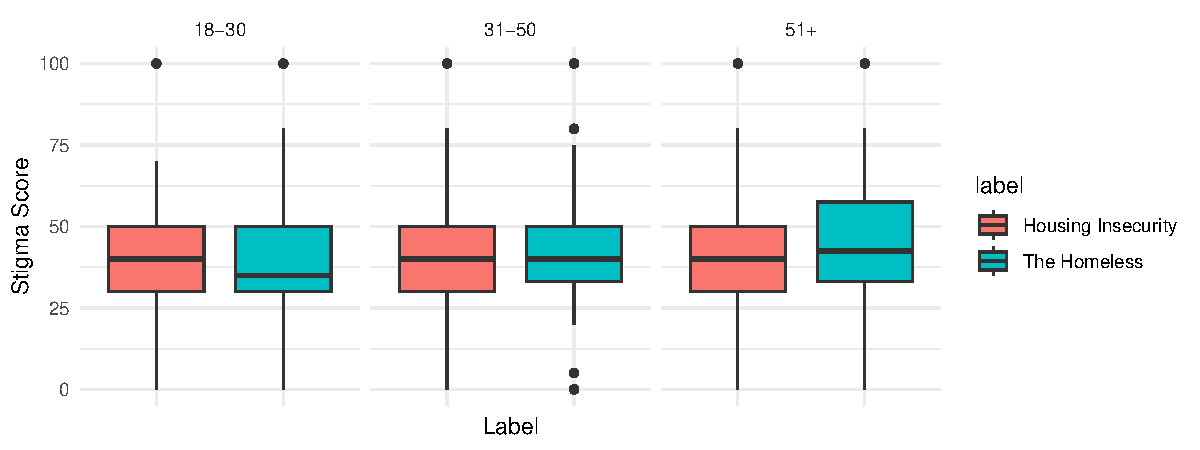
\includegraphics{00_PC_Label_Homeless_Results_files/figure-pdf/fig-donate-age-by-label-1.pdf}

}

\end{figure}%

\newpage

\section{References}\label{references}

\phantomsection\label{refs}
\begin{CSLReferences}{1}{0}
\bibitem[\citeproctext]{ref-fiskeetal_2002_model}
Fiske, S. T., Cuddy, A. J. C., Glick, P., \& Xu, J. (2002). A model of
(often mixed) stereotype content: {Competence} and warmth respectively
follow from perceived status and competition. \emph{Journal of
Personality and Social Psychology}, \emph{82}(6), 878--902.
\url{https://doi.org/10.1037/0022-3514.82.6.878}

\end{CSLReferences}






\end{document}
